\subsection{Muon Channel Selection}
\label{sec:muonid}

Muons candidates are first reconstructed separately in the central tracker (referred to simply as ``tracks'' or ``tracker tracks'')
and in the muon detector (``stand-alone muons''). Stand-alone muons are then matched and combined with tracker
tracks to form ``global muons''. Another independent algorithm proceeds from the central tracker outwards, matching
muon chambers hits and producing ``tracker muons''.

The following quality selection are applied to muon candidates.
Global and stand-alone muon candidates must have at least one good hit in the muon chambers.
Tracker muons must match to hits in at least two muon stations.
Tracks, global muons, and tracker muons must have more than 10 hits in the inner tracker, 
of which at least one must be in the pixel detector, and the impact parameter in the 
transverse plane, $d_{xy}$, calculated with respect to the beam axis, 
must be smaller than 2~mm.
More details and studies on muon identification can be found in Refs.~\cite{MUONPAS,MuonPerf}.
\begin{figure}
  \begin{center}
   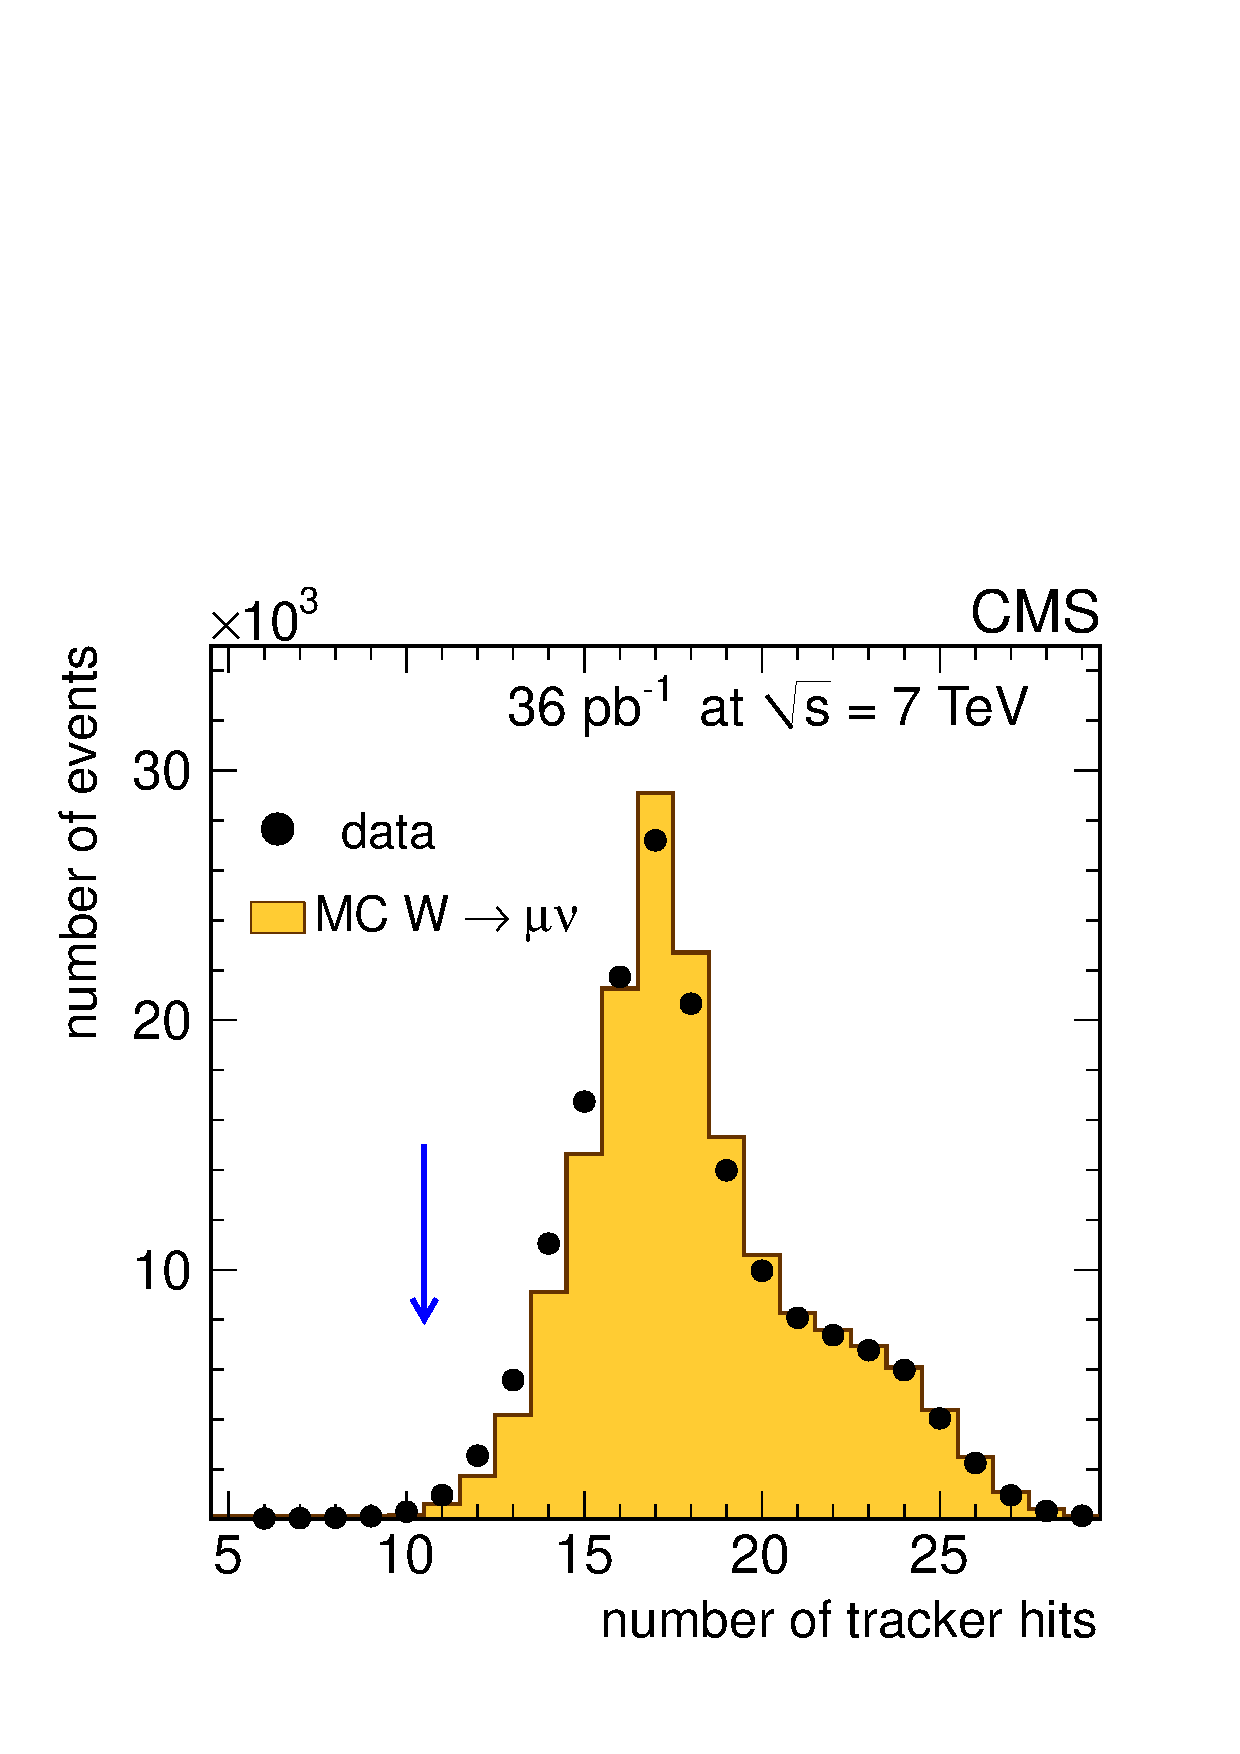
\includegraphics[width=0.39\textwidth]{figs/ntkhits.pdf}
   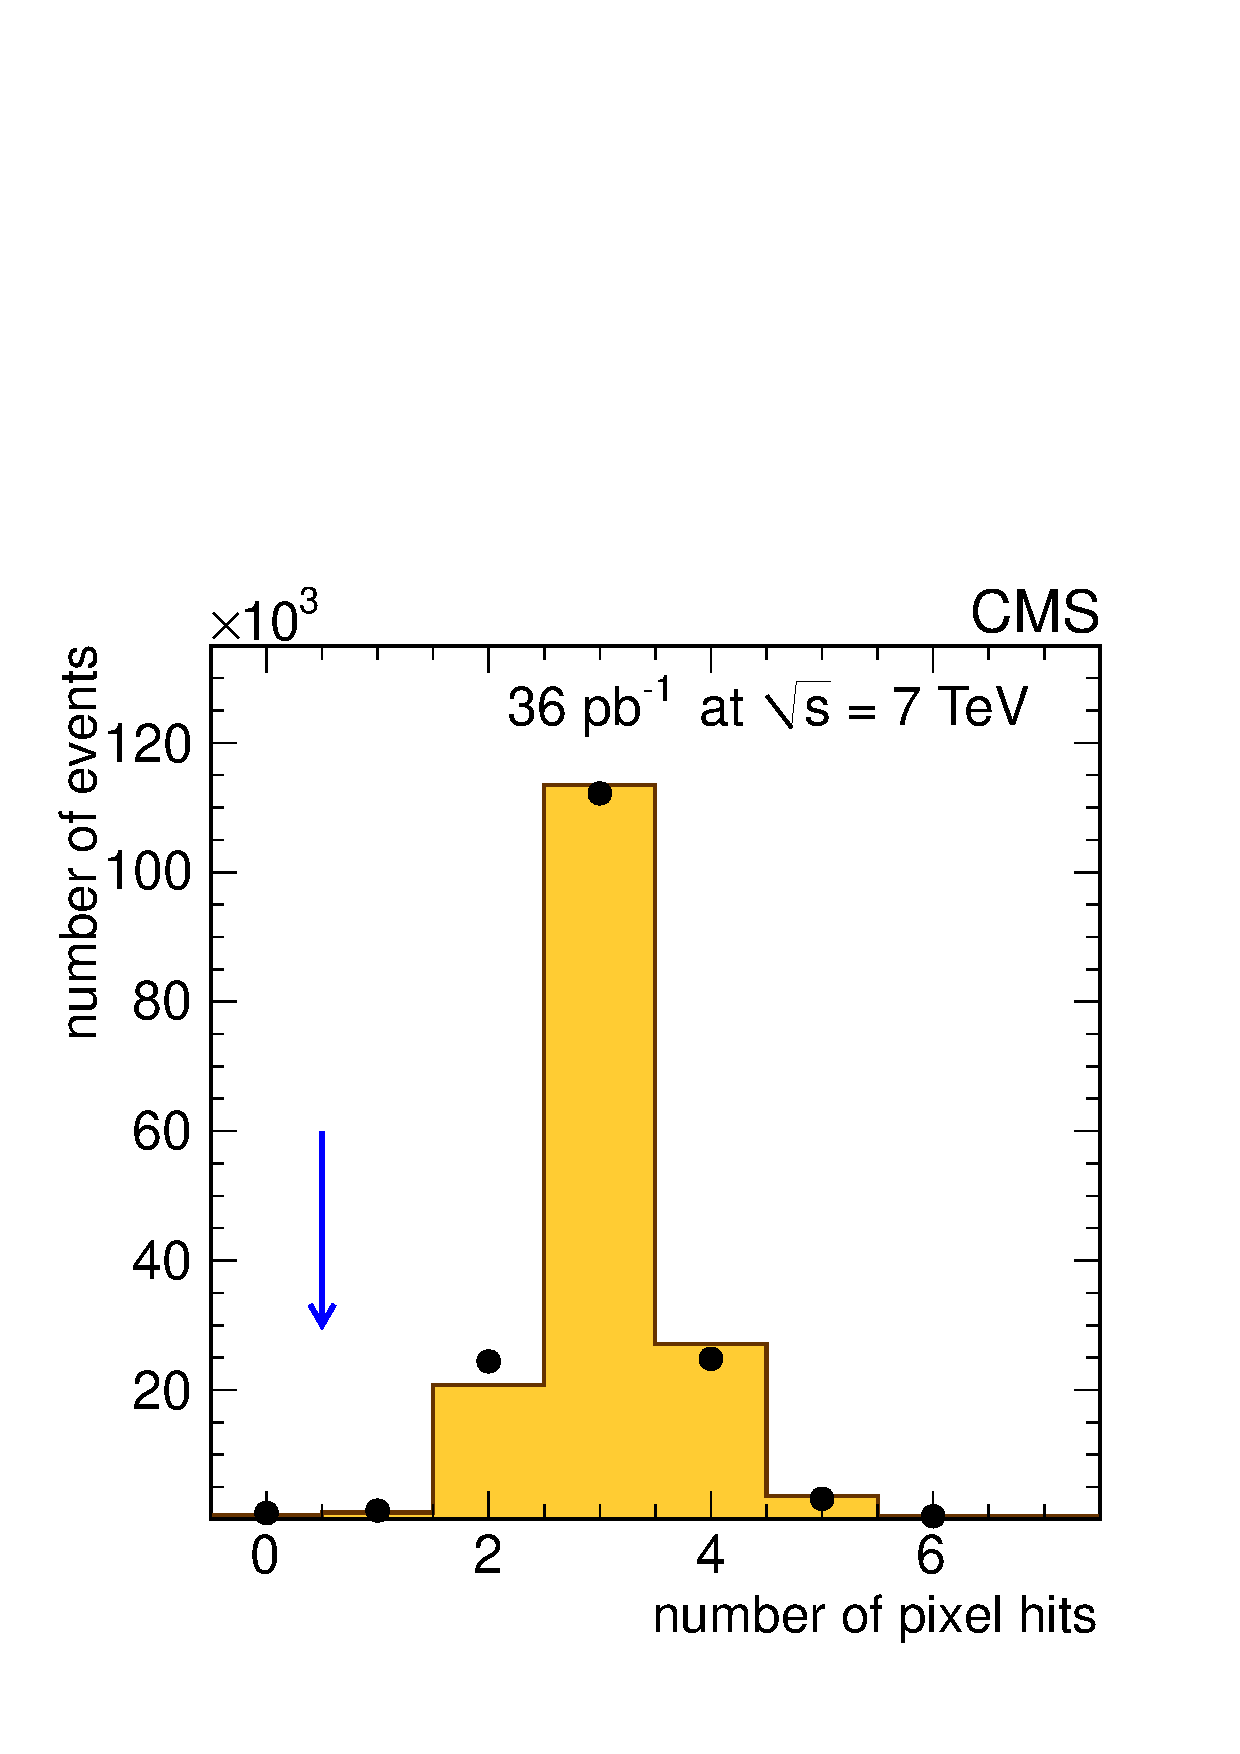
\includegraphics[width=0.39\textwidth]{figs/npixel.pdf}
   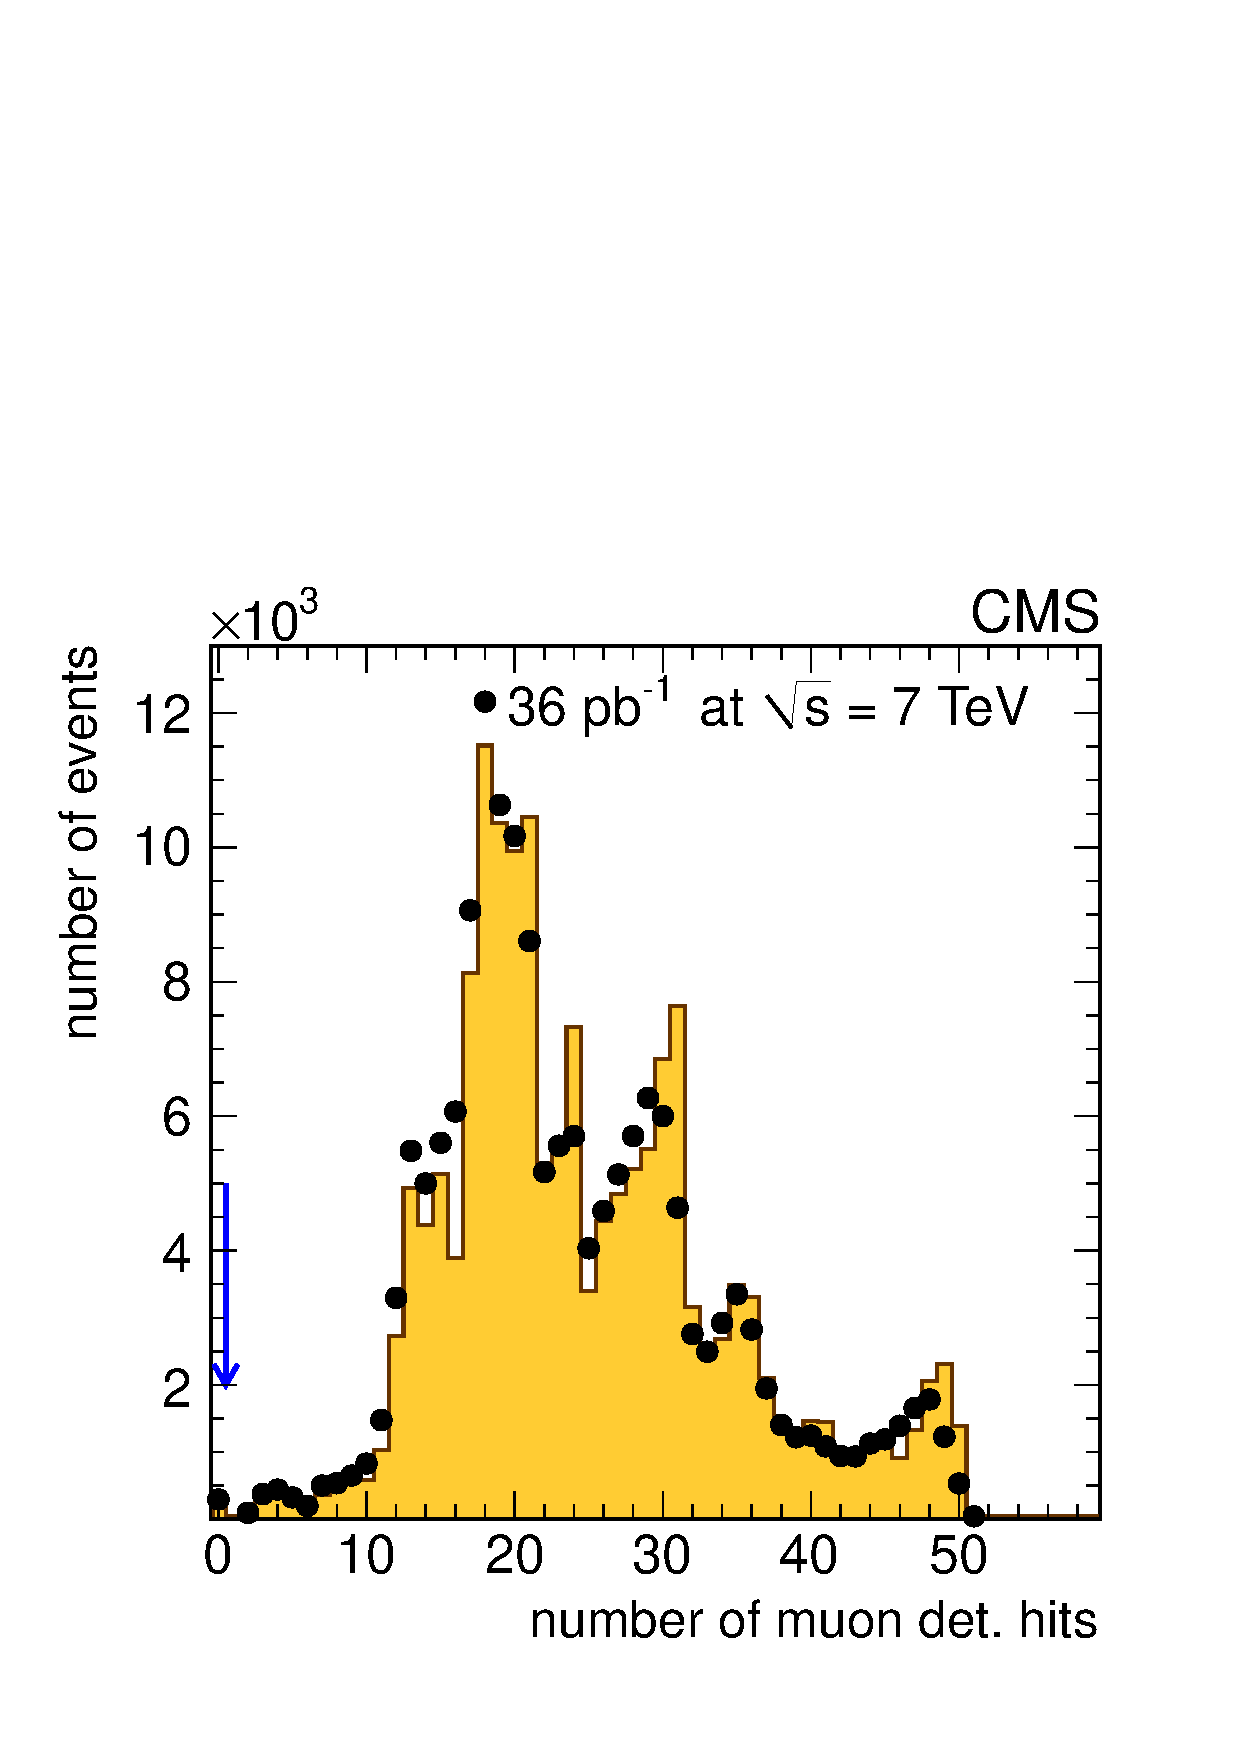
\includegraphics[width=0.39\textwidth]{figs/nmuons.pdf}
   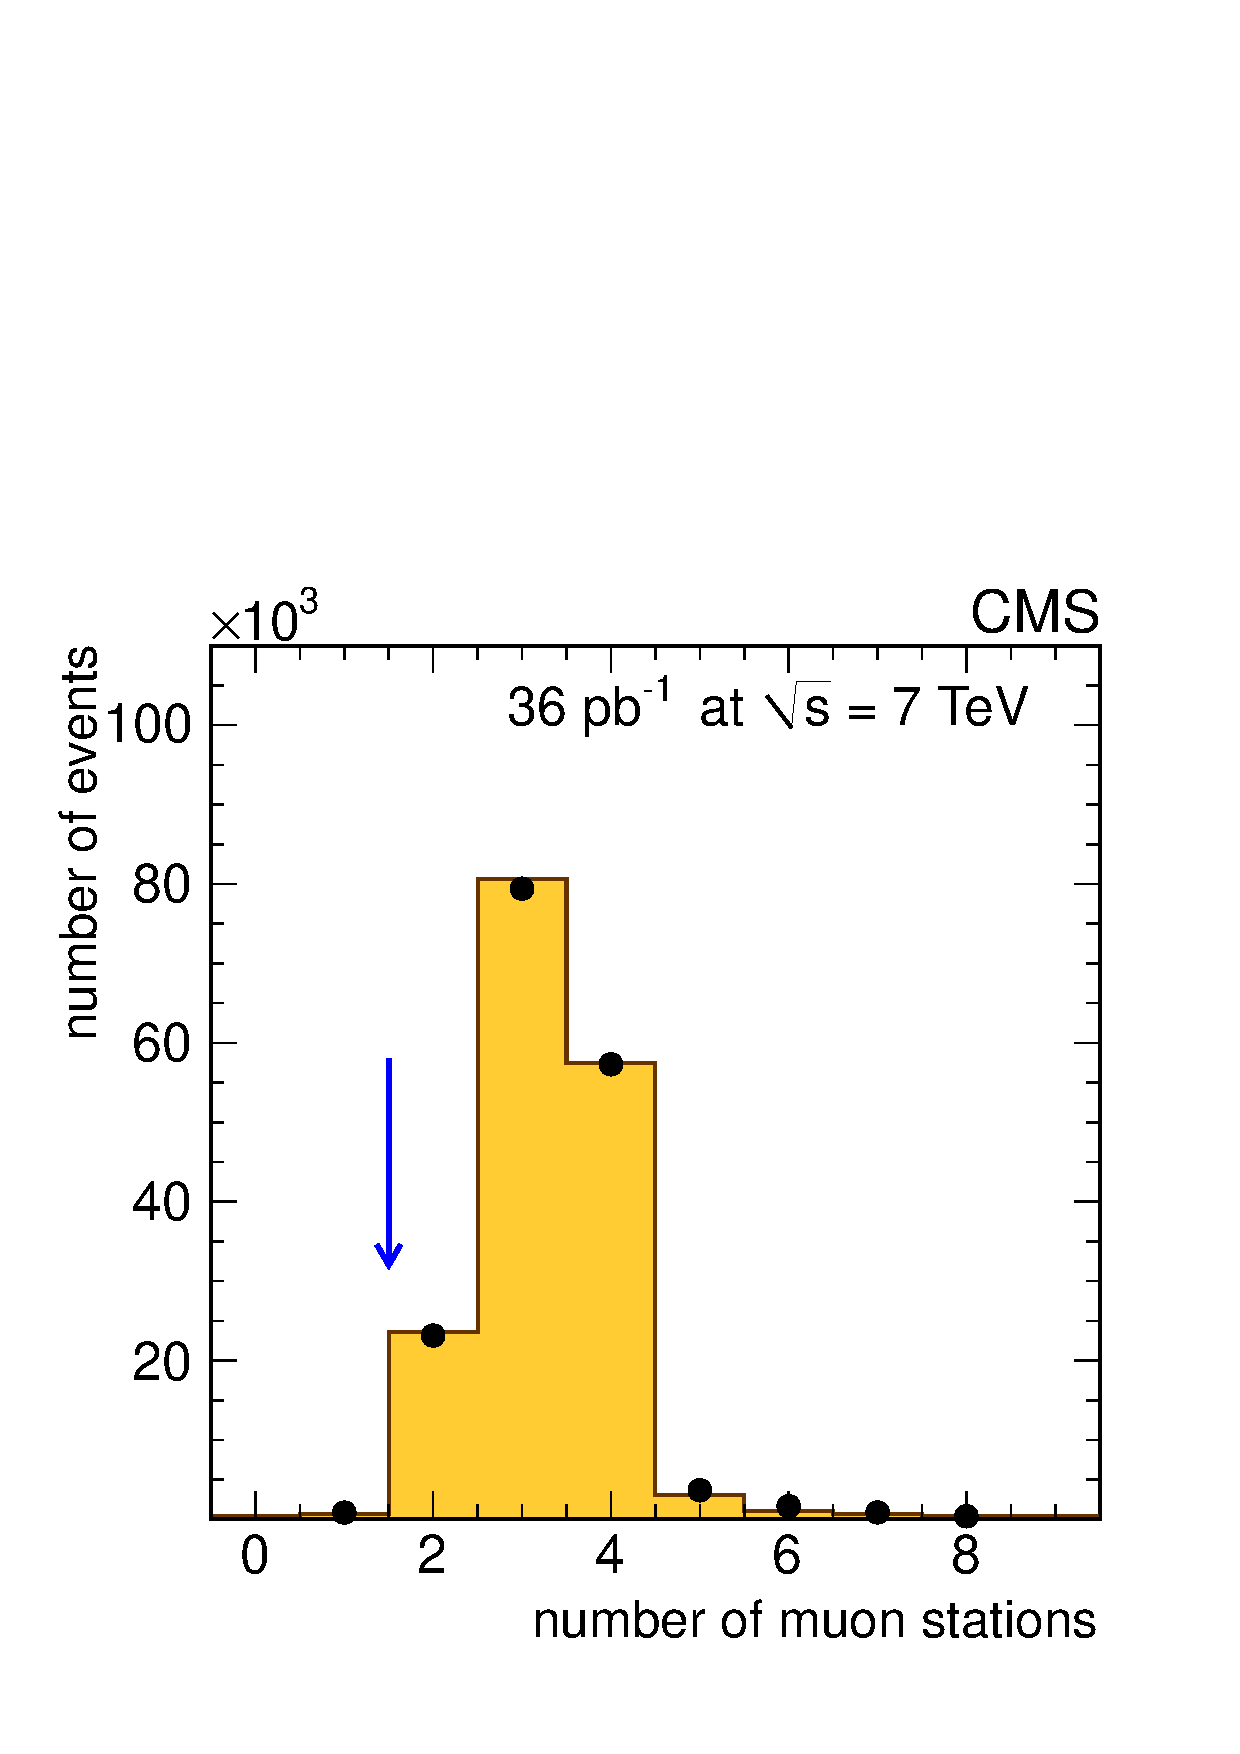
\includegraphics[width=0.39\textwidth]{figs/nmatches.pdf}
   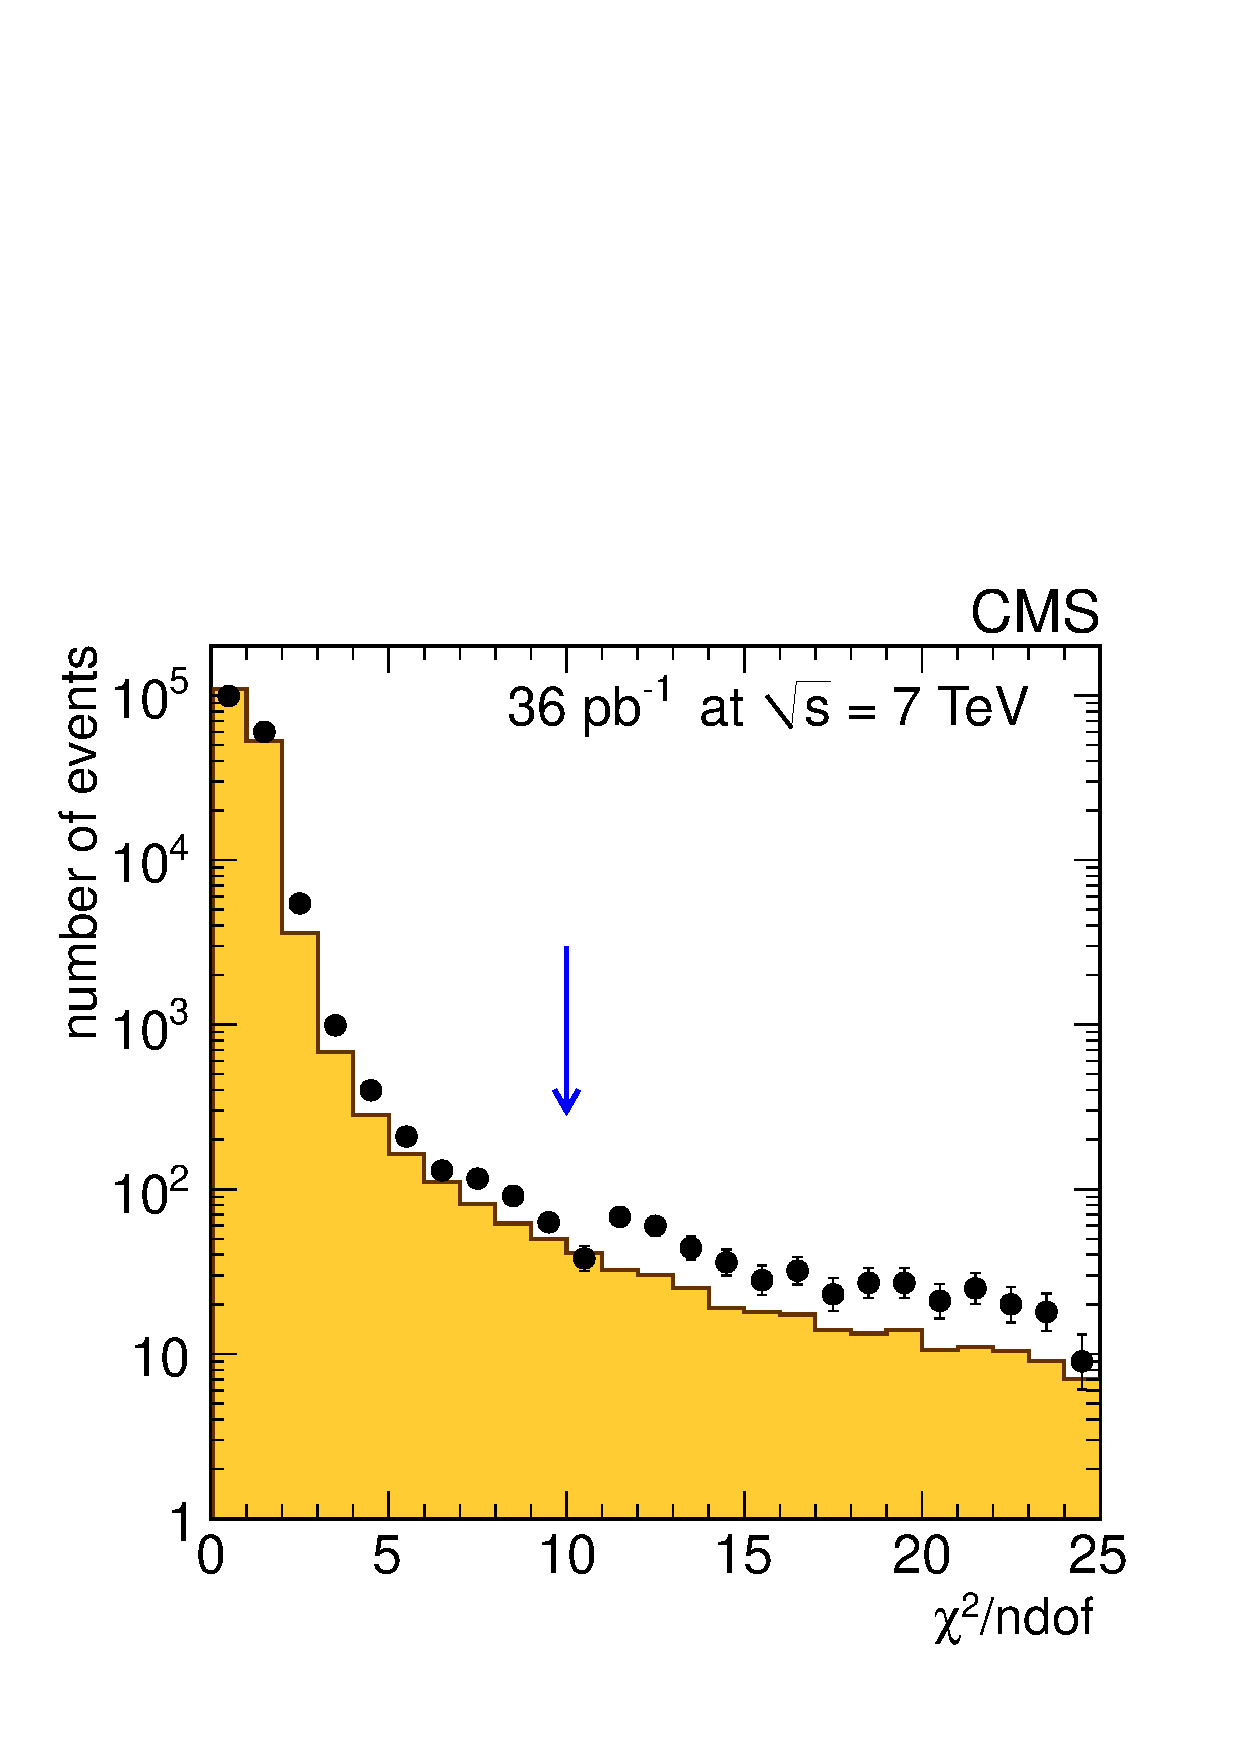
\includegraphics[width=0.39\textwidth]{figs/chi2_log.pdf}
   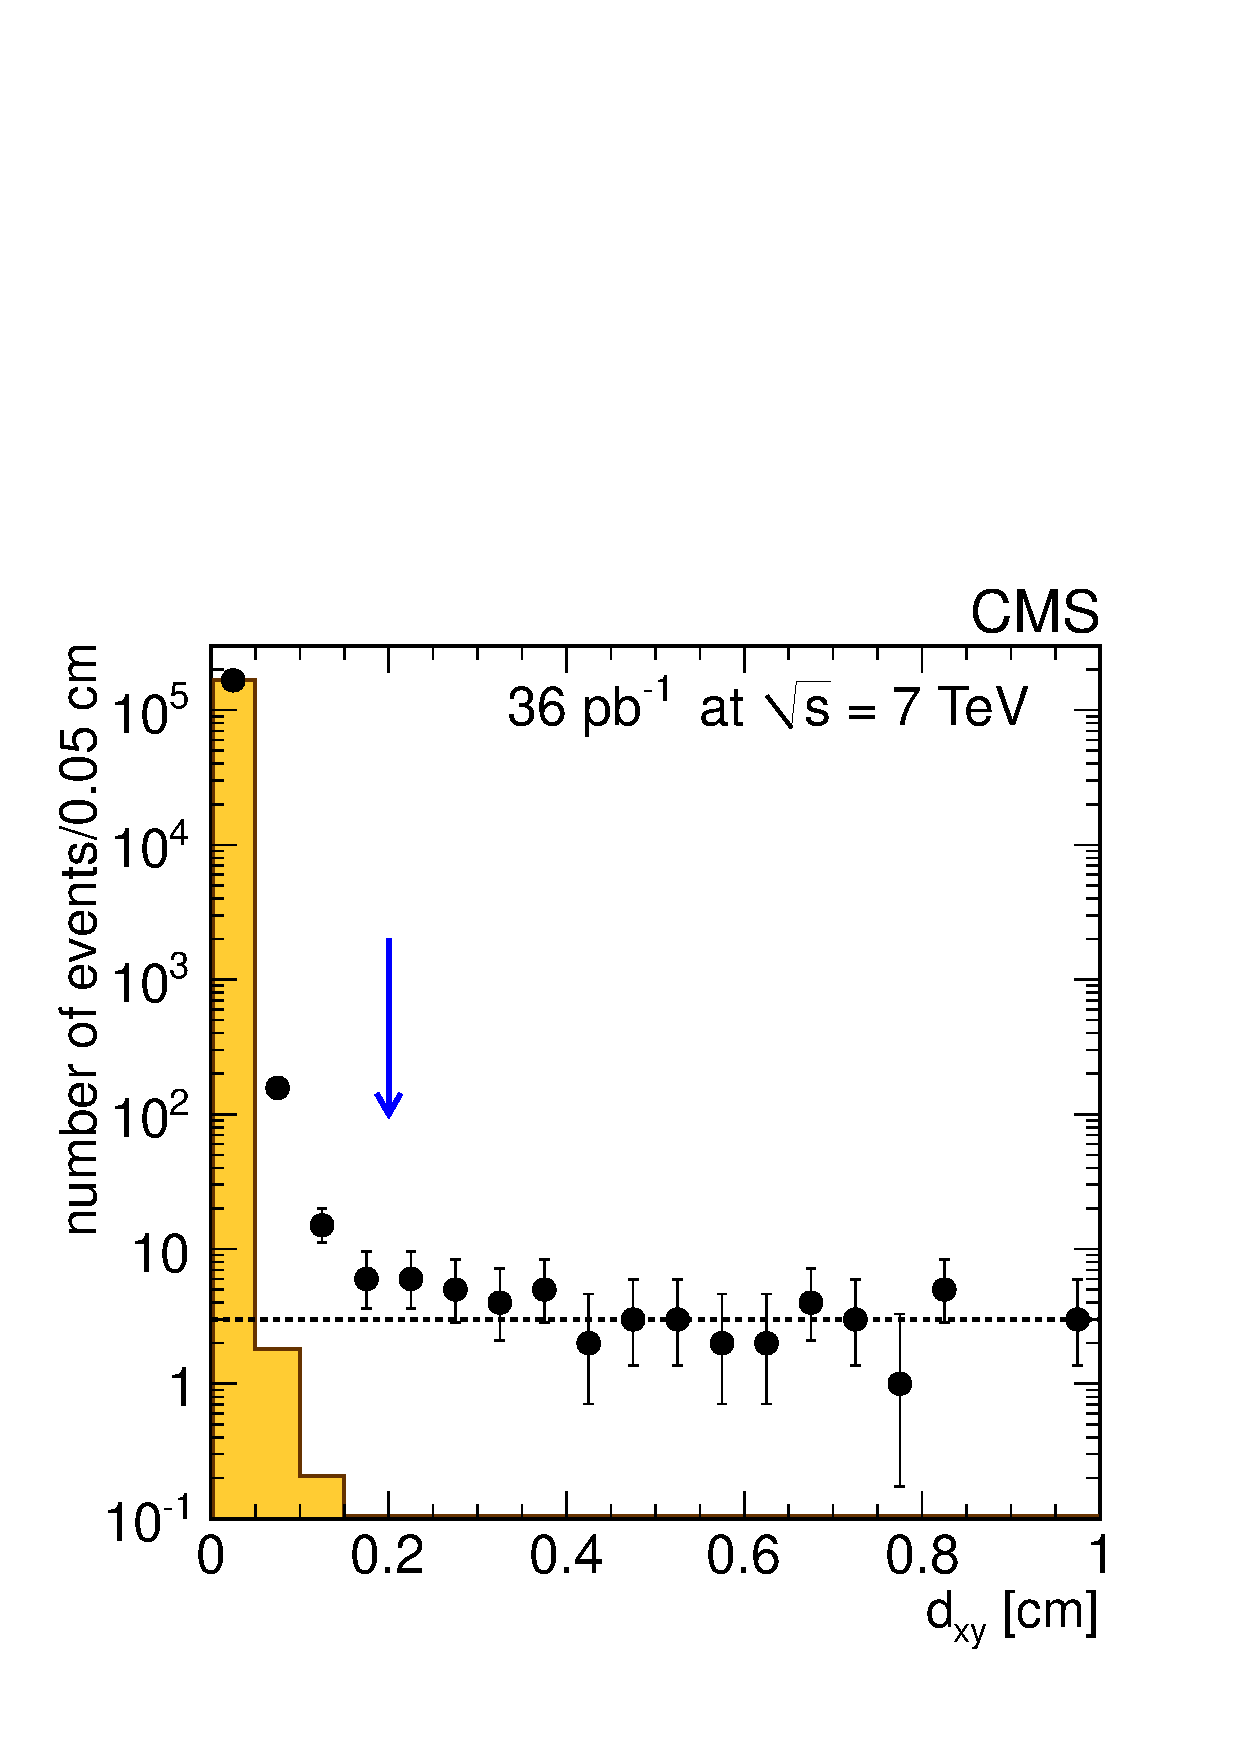
\includegraphics[width=0.39\textwidth]{figs/dxy_log.pdf}
   \caption{ \label{fig:muonIDvars}
Distribution of number of hits in the inner tracker and in the pixel detector,
number of hits in muon chambers, number of muon segments stations,
$\chi^2$ per degree of freedom, and transverse impact parameter $d_{xy}$ for data
(points with the error bars).
For illustration the simulated $\Wmn$ signal (histogram), normalized to the number of events 
observed in data, is superimposed.
These distributions are for events
satisfying all selection requirements, except that on
the presented variable.
The applied requirement on that variable is indicated as a blue arrow.
In the $d_{xy}$ distribution, the horizontal line shows the average of the 
bins with  $d_{xy}>0.2~\mathrm{cm}$
used to estimate the cosmic-ray muon contamination in the signal region.
The excess of events in data in the region with $d_{xy}<0.2~\mathrm{cm}$ with respect to $\Wmn$ 
signal simulation is due to muons from long-lived
particle decays in the QCD background.
}
  \end{center}
\end{figure}

Muon candidates selected in the $\Wmn$ analysis must be identified both as global and tracker muons.
Moreover, as additional quality selection, the global muon fit must have a $\chi^2$ per degree of freedom less than 10
in order to reject misidentified muons and misreconstructed particles.
The $\Wmn$ candidate events must have a muon candidate in the fiducial volume $|\eta|<2.1$ with 
$\Pt>25~\GeV$. 
The muon must be isolated, satisfying 
$\IRelComb = \left( \ITRK +\IECAL+\IHCAL\right)/\pt < 0.1$.
Events containing a second muon with $\Pt > 10~\GeV$ in the full muon acceptance region
($|\eta|<2.4$) are rejected to minimize the contamination from DY events.
The distributions of the variables used for muon quality selection are shown 
in Fig.~\ref{fig:muonIDvars} after applying all selection requirements, except that on
the presented  variable.

Background due to a cosmic-ray muon crossing the detector in coincidence with a pp collision is very
much reduced by the impact parameter requirement.
The remaining cosmic-ray background is evaluated by extrapolating to the signal region the rate of events with
large impact parameter.
Figure~\ref{fig:muonIDvars} (bottom, right) shows the distribution of the
impact parameter $d_{xy}$ for the $\Wmn$ candidates satisfying all selection requirements, except
that on $d_{xy}$.
Candidates with large $d_{xy}$ are mainly due to cosmic-ray muons and their rate is independent of $d_{xy}$.
A background fraction on the order of $10^{-4}$ in the $d_{xy}<2$~mm region is estimated.

The isolation distribution in data, together with the MC expectations, are shown in
Fig.~\ref{figure:Wmunu_iso}. 
\begin{figure}[htbp] {\centering
    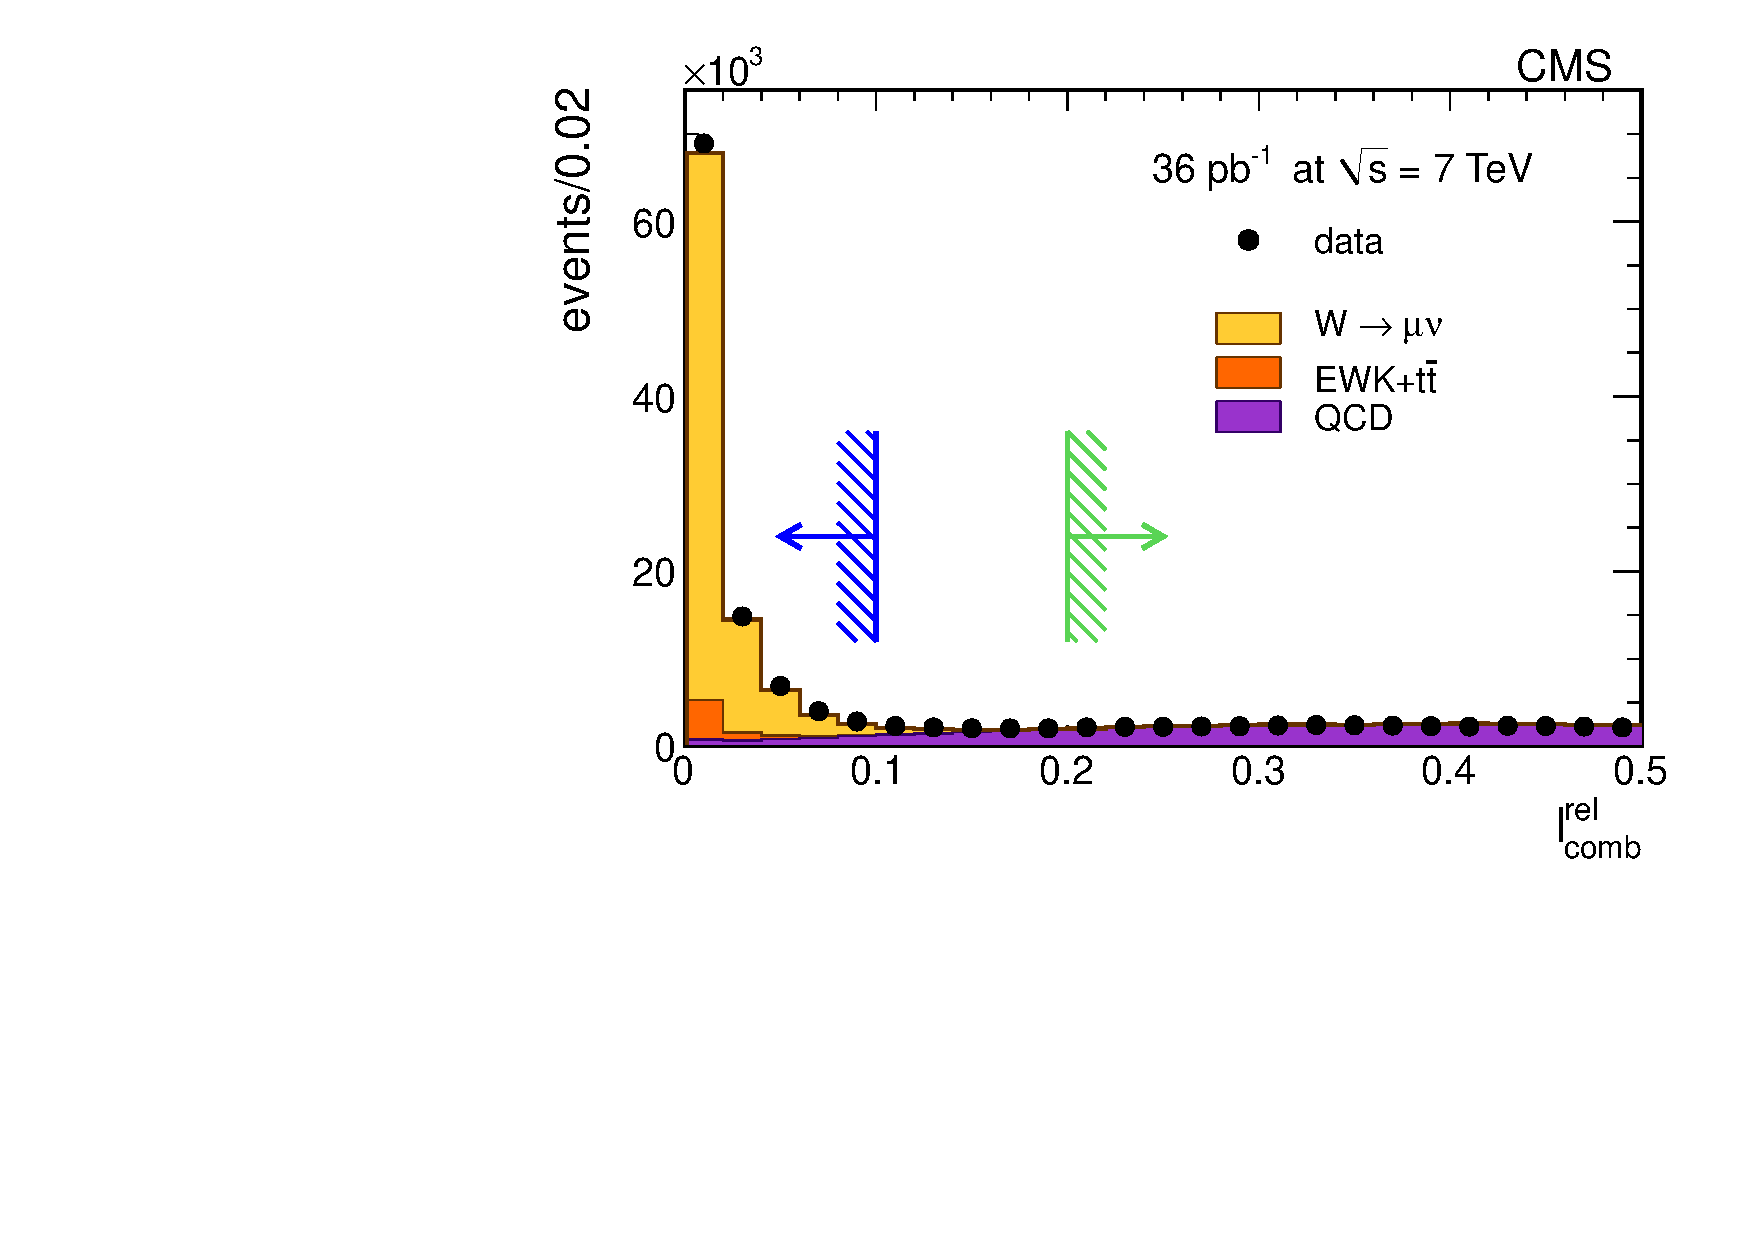
\includegraphics[width=0.5\textwidth]{figs/Wmunu_isolation.pdf}
    \caption{Distribution of $\IRelComb$ for candidates with a good quality muon 
      of $\Pt>25~\GeV$ in the fiducial region $|\eta|<2.1$.
      Points represent the data and the histograms the contribution from the 
      different SM processes.
      The signal selection requirement (dark blue arrow, $\IRelComb<0.1$) and the selection of the QCD-enriched
      control sample (light green arrow, $\IRelComb>0.2$) are shown.}
    \label{figure:Wmunu_iso}}
\end{figure}
Events with $\IRelComb > 0.2$ are mainly from QCD multijet background, and are used as
a control sample (Section~\ref{sec:WQCDbkg}).


% \begin{figure}[htbp] {
%     \centering
%     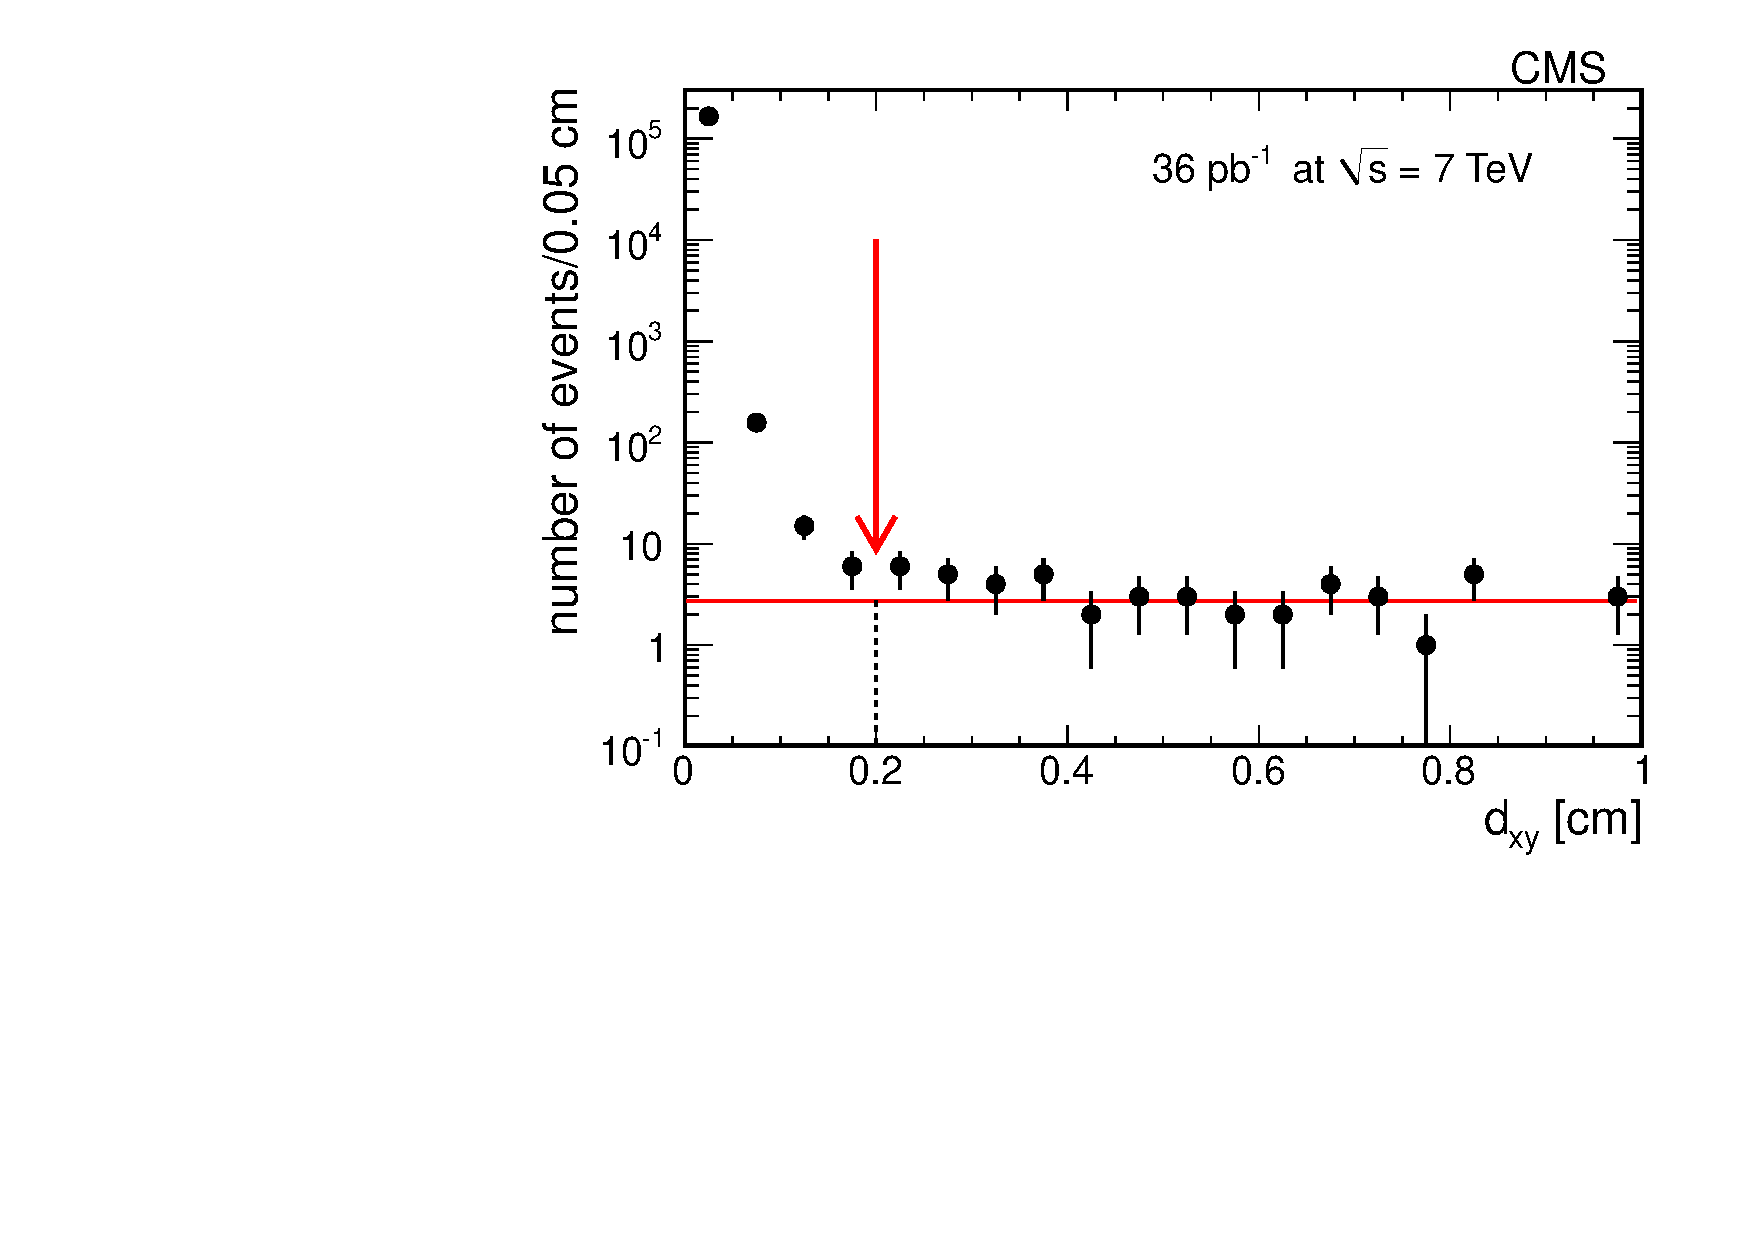
\includegraphics[width=0.5\textwidth]{figs/Wmn_cosmics.pdf}
%     \caption{Distribution of the transverse impact parameter $d_{xy}$ for the $\Wmn$
% candidates satisfying all selection requirements, except that on $d_{xy}$. 
% The vertical arrow shows the requirement applied to reject cosmic-ray muons.
% The horizontal line shows the average of the bins with  $d_{xy}>0.2~\mathrm{cm}$
% used to estimate the (negligible) cosmic contamination in the signal region.
%     \label{figure:Wmn_muon_dxy}}
% }
% \end{figure}


After the selection process described, 166\,457 events are selected,
97\,533 of them with a positively charged muon candidate and 68\,924 with a negatively
charged muon candidate.

$\Zmm$ candidate events are selected by pairing a global muon matched to an HLT trigger muon with a second
oppositely charged muon candidate that can be either a global muon, a stand-alone muon, or a track. 
No $\chi^2$ selection or requirement that the muon be reconstructed 
through the tracker-muon algorithm is applied. 
The two muon candidates must both have $\Pt > 20~\mathrm{GeV}$ and $|\eta| < 2.1$,
and their invariant mass must be in the range $60<m_{\mu\mu}<120$~$\mathrm{GeV}$.
Both muon candidates must be isolated according to the tracker isolation requirement $\ITRK<3$~GeV.
The different choice of isolation requirements in $\Wmn$ and $\Zmm$ is
motivated in Section~\ref{sec:Zmumu}.
After the selection process, the number of selected events with two
global muons is 13\,728.
